\chapter{Simple Intuitive Model for Potentials} \label{chap:SIMP}
The following chapter introduces a simple intuitive model for potentials (\emph{SIMP}) for both the coplanar capacitor and the $p$-$n$-junction, as well as its comparison with FEM simulations and experimental results obtained through off-axis electron holography and tomography.
\section{Mathematical Foundations}
Most software packages use some form of FEM (utilizing a mesh-based approach) for solving the Poisson (partial differential) equation, making such simulations computationally complex. The following \cref{ssec:classical-electrostatics} gives a brief insight into the Poisson equation and its solution using Green's function, while \cref{ssec:SIMP-alternative-model} derives an alternative model for the description of such electrostatic potentials in complex real-world specimens.
\subsection{Classical Electrostatics} \label{ssec:classical-electrostatics}
One of the foundations of electrostatics involves solving the Poisson equation:
\begin{equation}
  \laplacian \phi \left(\vb{r}\right) = -\frac{\rho\left(\vb{r}\right)}{\epsilon_0}
\end{equation}
for a given charge carrier density $\rho\left(\vb{r}\right)$ \cite{Jackson1999}. The solution for the scalar electrostatic potential is therefore given by:
\begin{equation}
  \phi \left(\vb{r}\right) = \frac{1}{4\pi \epsilon_0} \int \frac{\rho\left(\vb{r'}\right)}{\lvert \vb{r} - \vb{r'}\rvert} \dd{\vb{r'}} = \frac{1}{4\pi \epsilon_0} \int \rho\left(\vb{r'}\right) G_0\left(\vb{r}, \vb{r'}\right) \dd{\vb{r'}},
\end{equation}
where $G_0\left(\vb{r}, \vb{r'}\right) = \lvert \vb{r} - \vb{r'}\rvert^{-1}$ is the free space Green's function yielding the response at point $\vb{r}$ due to a point charged placed at $\vb{r'}$ \cite{Jackson1999}.

Using the Poisson equation for such a point charge yields \cite{Jackson1999}:
\begin{equation}
  \laplacian \frac{1}{\lvert \vb{r} - \vb{r'}\rvert} = \laplacian G_0\left(\vb{r}, \vb{r'}\right) = -4\pi \delta\left(\vb{r} - \vb{r'}\right).
\end{equation}
Considering that charges can collect on a surface $S$ of a volume $V$ with given boundary conditions, Green's second identity can be used to find the solution as:
\begin{align}
  \label{eq:electrostatic-poisson-green}
  \phi \left(\vb{r} \in V \right) & = \frac{1}{4\pi \epsilon_0} \int \limits_V \rho\left(\vb{r'}\right) G_0\left(\vb{r}, \vb{r'}\right) \dd{\vb{r'}} \notag \\
  &+ \frac{1}{4\pi} \oint \limits_S \left[ G_0\left(\vb{r}, \vb{r'}\right) \pdv{\phi \left(\vb{r'}\right)}{n'} - \phi \left(\vb{r'}\right) \pdv{G_0\left(\vb{r}, \vb{r'}\right)}{n'} \right] \dd{S'},
\end{align}
where the unit normal $\vb{n'}$ points outwards from $V$ \cite{Jackson1999}.

While \cref{eq:electrostatic-poisson-green} might yield a correct solution in the context of electrostatic problems, it requires extensive knowledge about the charge carrier distribution and boundary conditions, something which is rarely known for complex specimens. Therefore, a simple and intuitive model utilizing the convolution of a initial potential distribution with a 1D~Gaussian kernel is developed (\cref{fig:SIMP-basic-idea}).
\subsection{Alternative Model} \label{ssec:SIMP-alternative-model}
Assuming a charge-free distribution for $z > 0$ (i.\,e.\ outside the specimen), the Poisson equation for the 3D~electrostatic potential $\phi\left(\vb{r}\right)$ is reduced to the Laplace equation \cite{Jackson1999}:
\begin{equation}
  \laplacian{\phi\left(\vb{r}\right)} = 0 \quad \forall\, \vb{r} \in \left\{\mathbb{R}^3\, \middle| \, z > 0\right\}.
\end{equation}
If distribution in $y$-direction is either homogenous or infinitely large, the 3D~problem is reduced to 2D:
\begin{equation}
	\label{eq:poisson-equation-2D-approximation}
  \left(\partial^2_x + \partial^2_z\right)\phi\left(x, z \right) = 0 \quad \forall\, x, z \in \left\{\mathbb{R}\, \middle| \, z > 0\right\},
\end{equation}
where the 2D~electrostatic potential at $z = 0$ (i.\,e.\ at the edge of the specimen) is given by the initial electrostatic potential distribution $\phi_0 \left(x\right)$:
\begin{equation}
  \phi\left(x, 0\right) = \phi_0 \left(x\right).
\end{equation}
The solution is then given by the Green's function with Dirichlet boundary conditions:
\begin{equation}
  G\left(x, x', z, z'\right) = G\left(x, x', z, z'\right) + F\left(x, x', z, z'\right),
\end{equation}
where both functions satisfy the condition \cite{Jackson1999}:
\begin{equation}
  G\left(x, x', z, 0\right) = 0 \quad ; \quad \laplacian{F\left(x, x', z, z'\right)} = 0.
\end{equation}
The function $F\left(x, x', z, z'\right)$ can be chosen arbitrarily due to the Green's function being invariant under gauge transformations (as long as the gauge invariance is not violated) \cite{Jackson1999}.

The solution for the 2D~electrostatic potential is then given (following \cref{eq:electrostatic-poisson-green}) by \cite{Jackson1999}:
\begin{align}
	\label{eq:2D-electrostatic-poisson-green}
  \phi\left(x, z\right) &= \int G\left(x, x', z, z'\right) \rho\left(x', z'\right) \dd{x'} \dd{z'} \nonumber \\
  &- \int \phi_0\left(x'\right) \underbrace{\eval{\pdv{G\left(x, x', z, z'\right)}{z'}}_{z' = 0}}_{\coloneqq \widetilde{G}\left(x, x', z'\right)} \dd{x'},
\end{align}
where the first integral vanishes because the charge carrier distribution $\rho\left(x', z'\right)$ is zero outside the specimen.
\begin{figure}[H]
	\centering
	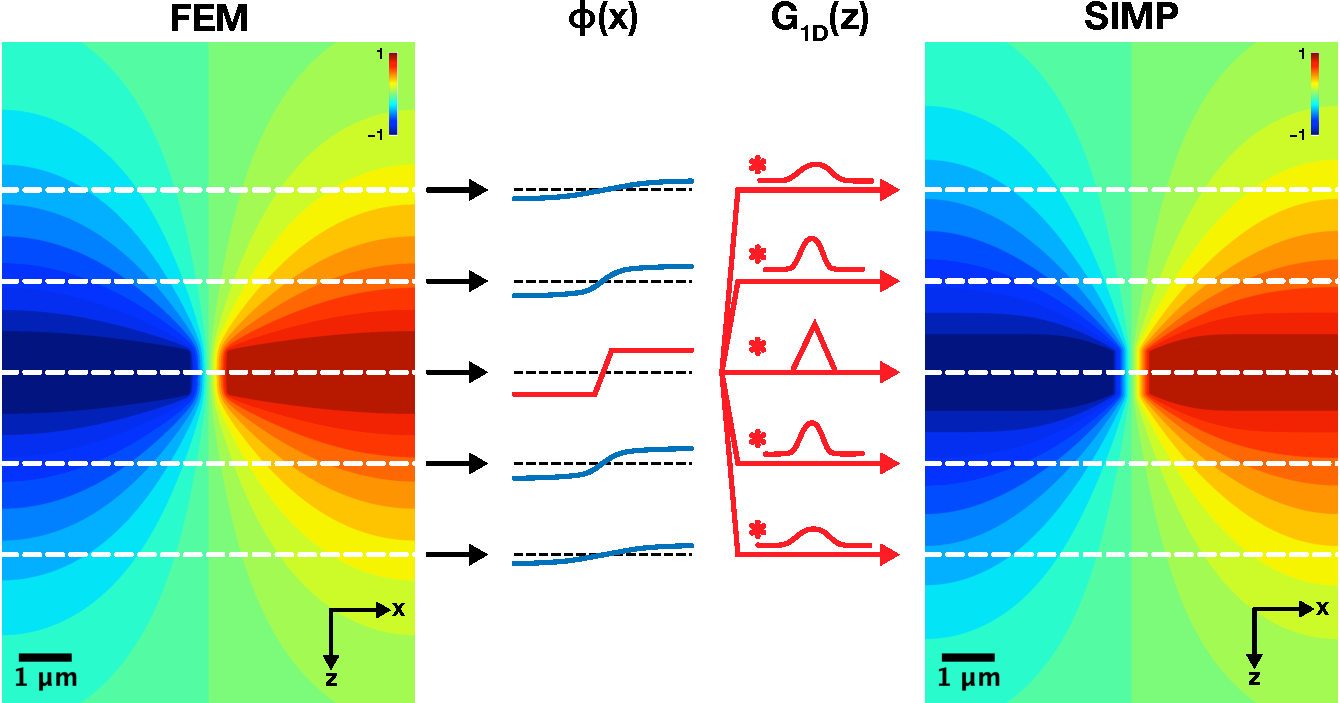
\includegraphics[width=\textwidth]{Figures/Schematics/SIMP-basic-idea.pdf}
	\caption{Schematic illustration of the mathematical foundation behind \emph{SIMP}. The line profiles $\phi\left(x\right)$ (indicated by the dashed white lines) of the 2D~electrostatic potential $\phi$ obtained from FEM simulations show the expected behavior at different projection distances $z$ from the specimen. Taking the initial electrostatic potential distribution $\phi_0\left(x\right)$ (red curve) and calculating the convolution with a projection distance dependent (normalized) 1D Gaussian kernel $G_{\mathit{1D}}\left(z\right)$ according to \cref{eq:SIMP-electrostatic-potential-convolution} yields a similar 2D~electrostatic potential.}
	\label{fig:SIMP-basic-idea}
\end{figure}
Furthermore, $\widetilde{G}\left(x, x', z'\right)$ has to obey the boundary conditions:
\begin{equation}
	\eval{\phi\left(x, z\right)}_{z \to \infty} = \text{const.} \quad ; \quad \eval{\phi\left(x, z\right)}_{z = 0} = \phi_0 \left(x\right),
\end{equation}
which therefore means that:
\begin{equation}
	\label{eq:green-function-boundary-conditions}
	\eval{\widetilde{G}\left(x, x', z'\right)}_{z \to \infty} = \text{const.} \quad ; \quad \eval{\widetilde{G}\left(x, x', z'\right)}_{z \to 0} = \delta \left(x - x'\right).
\end{equation}
The (normalized) Gaussian distribution can be described as a delta sequence \cite{Jackson1999} whose standard deviation obeys $\eval{\sigma_G}_{z \to 0} = 0$ and therefore the second condition of \cref{eq:green-function-boundary-conditions}. Additionally, the first condition of \cref{eq:green-function-boundary-conditions} is trivially fulfilled by the Gaussian distribution.

Given an initial electrostatic potential distribution $\phi_0 \left(x\right)$, the 2D~electrostatic potential can therefore be calculated (according to \cref{eq:2D-electrostatic-poisson-green}) through a convolution:
\begin{equation}
  \label{eq:SIMP-electrostatic-potential-convolution}
  \phi \left(x, z\right) = \phi_0\left(x\right) * G_{\mathit{1D}}\left(z\right),
\end{equation}
where $G_{\mathit{1D}}\left(z\right)$ is a 1D~Gaussian kernel. Here, the standard deviation $\sigma_G$ of the convolution kernel is dependent on the projection distance $z$ and scales with a power of $\ln\left(2\right)$ inside the stray field.

\emph{SIMP} consequently allows for the description of complex electrostatic problems, requiring minimal knowledge of the specimen besides an initial electrostatic potential distribution (which is given through simple analytical formulas for most geometric layouts and specimens) while significantly cutting down on computational complexity. Additionally, \emph{SIMP} offers the advantage that the computation of the 2D~electrostatic potential is done row by row, where each $\phi \left(x, z\right)$ does not depend on the previous result, allowing the computation to be parallelized and scale linearly with the available computational power.
\newpage
\section{Coplanar Capacitor} \label{sec:coplanar-capacitor-SIMP-EH-comparison}
In order to verify the validity of the presented model, the coplanar capacitor (\cref{fig:specimen-capacitor-layout}) described in \cref{ssec:2d-modeling-specimen}, whose physical behavior is well understood, is modeled and compared using both FEM simulations and \emph{SIMP}. These findings are used to compare the results obtained from \emph{SIMP} with experimental data obtained from off-axis EH and electron tomography.
\subsection{Comparison with Finite Element Method Simulations}
Due to the axial symmetry, only half of the problem's geometry, as described in \cref{ssec:2d-modeling-specimen}, needs to be modeled using FEM simulations and \emph{SIMP} (\cref{fig:capacitor-FEM-SIMP-comparison}), where appropriate adjustments were again made to account for the symmetry of the problem.
\begin{figure}[H]
	\centering
	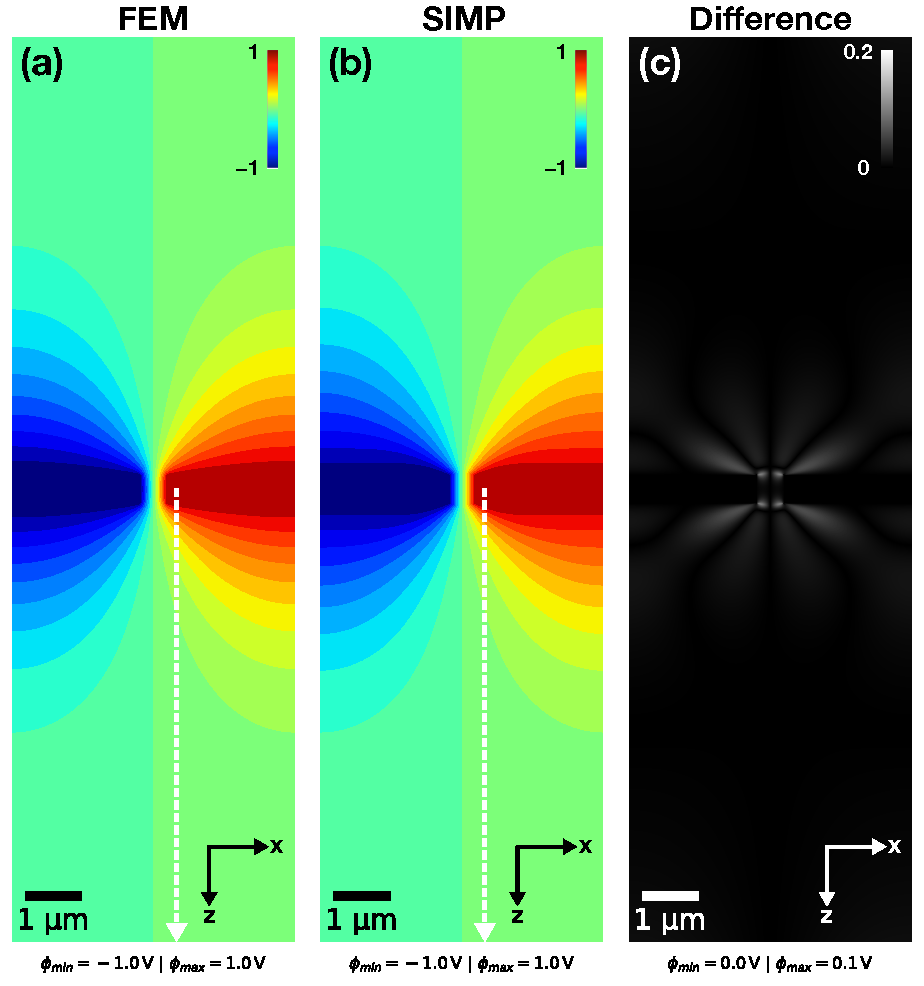
\includegraphics[width=0.8\textwidth]{Figures/Results/Capacitor/Simulations/capacitor-FEM-SIMP-comparison.pdf}
	\caption{Comparison between the 2D~electrostatic potential $\phi$ of the coplanar capacitor obtained from (a) the FEM simulation and (b) \emph{SIMP} along with (c) their absolute difference.}
	\label{fig:capacitor-FEM-SIMP-comparison}
\end{figure}
The electrostatic potential within the specimen region (i.\,e.\ for $\lvert z \rvert \le t = \SI{250}{\nm}$) is fully defined by the initial electrostatic potential distribution $\phi_0\left(x\right)$. Here, $\phi_0\left(x\right)$ is comprised of a constant potential $\phi_0\left(x\right) = \pm U_{\mathit{ext}}$ within the contacts and a linear slope between them. For $\lvert z \rvert \le t = \SI{250}{\nm}$ (i.\,e.\ for propagation distances starting at the specimen edge and extending into the vacuum region), $\phi \left(x, z\right)$ is calculated according to \cref{eq:SIMP-electrostatic-potential-convolution} from a convolution with a propagation distance dependent Gaussian kernel, where the kernel scales with a power of $\ln\left(2\right)$ and the standard deviation $\sigma_G$ ranges from $\sigma_G^{\mathit{min}} = \SI{1}{\nm}$ to $\sigma_G^{\mathit{max}} = \SI{4000}{\nm}$.

By comparing the 2D~electrostatic potential $\phi$ obtained from the FEM simulation (\cref{fig:capacitor-FEM-SIMP-comparison}a) with the one obtained from \emph{SIMP} (\cref{fig:capacitor-FEM-SIMP-comparison}b), it is apparent that presented model is in excellent agreement with well established simulation methods. As in the case with the FEM simulation, it is evident that the stray field extends well beyond the edge of the specimen into the vacuum region. Furthermore, by calculating the absolute difference of the two electrostatic potentials (\cref{fig:capacitor-FEM-SIMP-comparison}c), it is observed that the maximum deviation of $\Delta \phi_{\mathit{max}} = \SI{0.1}{\volt}$ is limited only to an area close to the contacts, where the approximations made in \cref{eq:poisson-equation-2D-approximation} are no longer valid for small $z$.
\newpage
Similar to \cref{ssec:experimental-results-capacitor-FEM-simulation}, the phase $\varphi$ can be obtained from the projection of the electrostatic potential (\cref{fig:capacitor-FEM-SIMP-linescan-comparison}a). Here it is evident that the phases (without any weighting applied to the different specimen regions), which were both offset to zero through subtraction by the first value, likewise exhibit minimal deviations. As already noted in \cref{ssec:experimental-results-capacitor-FEM-simulation}, the specimen (i.e. the region inside and between the contacts) only contributes a small part to the total phase (approximately 8\% of the maximum phase shift), which is predominantly made up of the stray field contribution. Additionally, the line profiles $\phi\left(z\right)$ of the electrostatic potential in propagation direction (indicated by the white dashed lines in \cref{fig:capacitor-FEM-SIMP-comparison}a and b) also demonstrate excellent agreement between the FEM simulation and \emph{SIMP}, with both line profiles approaching $\lim_{z\to\SI{8000}{\nm}} \phi\left(z\right) = \SI{0}{\volt}$.
\begin{figure}[H]
	\centering
	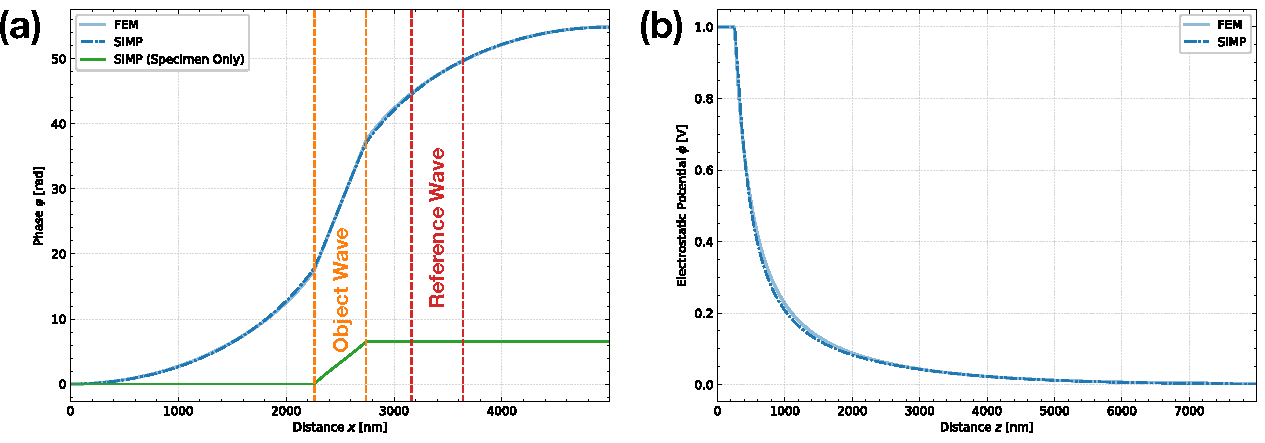
\includegraphics[width=\textwidth]{Figures/Results/Capacitor/Simulations/capacitor-FEM-SIMP-linescan-comparison.pdf}
	\caption{Comparison between the FEM simulation and \emph{SIMP} for the coplanar capacitor with (a) the phases $\varphi$ obtained through a projection of the 2D~electrostatic potential $\phi$ (with the object and reference wave indicated by the dashed orange and red lines) and (b) the line profiles $\phi\left(z\right)$ of the electrostatic potential in propagation direction (indicated by the white dashed lines in \cref{fig:capacitor-FEM-SIMP-comparison}a and b).}
	\label{fig:capacitor-FEM-SIMP-linescan-comparison}
\end{figure}
Considering the line profiles in \cref{fig:capacitor-FEM-SIMP-linescan-comparison}b, it is evident that the electrostatic potential calculated with \emph{SIMP} features the expected decay proportional to $1/z$. Furthermore, the plateau region at the beginning of both line profiles reflects the constant potential for $\lvert z \rvert \le t = \SI{250}{\nm}$ given from the initial potential distribution $\phi_0 \left(x\right)$, where the origin $z_0 = \SI{0}{\nm}$ for both line profiles lies precisely in the middle of the contacts.

Examining the line profiles further confirms the aforementioned findings, where the stray field extends well beyond the specimen edge into the vacuum region and accounts for much of the overall phase, with the electrostatic potential dropping to 10\% of its initial value of $U_{\mathit{ext}} = \pm \SI{1.0}{\volt}$ after a propagation distance of $z \approx \SI{2000}{\nm}$.

While the agreement between the FEM simulation and \emph{SIMP} for an identical specimen geometry seems promising at first, the question of the robustness of the presented model still arises. In order to verify this, it is investigated whether the same excellent agreement is achieved for a modified specimen geometry, all other parameters being equal.
\newpage
For this purpose, the distance between the capacitor plates $d$, with otherwise unchanged specimen geometry and simulation parameters, is modified to $d = \SI{960}{\nm}$ and $d = \SI{240}{\nm}$ (i.\,e.\ exactly double and half the above described distance $d$), respectively, and the deviation between the two models is investigated (\cref{fig:capacitor-FEM-SIMP-comparison-varying-distance}). To be precise, it is of interest whether a modified specimen geometry continues to produce the small deviations observed above between the two models while keeping the parameters with respect to the standard deviation of the Gaussian kernel $\sigma_G$ and the initial electrostatic potential distribution $\phi_0\left(x\right)$ unchanged.
\begin{figure}[H]
	\centering
	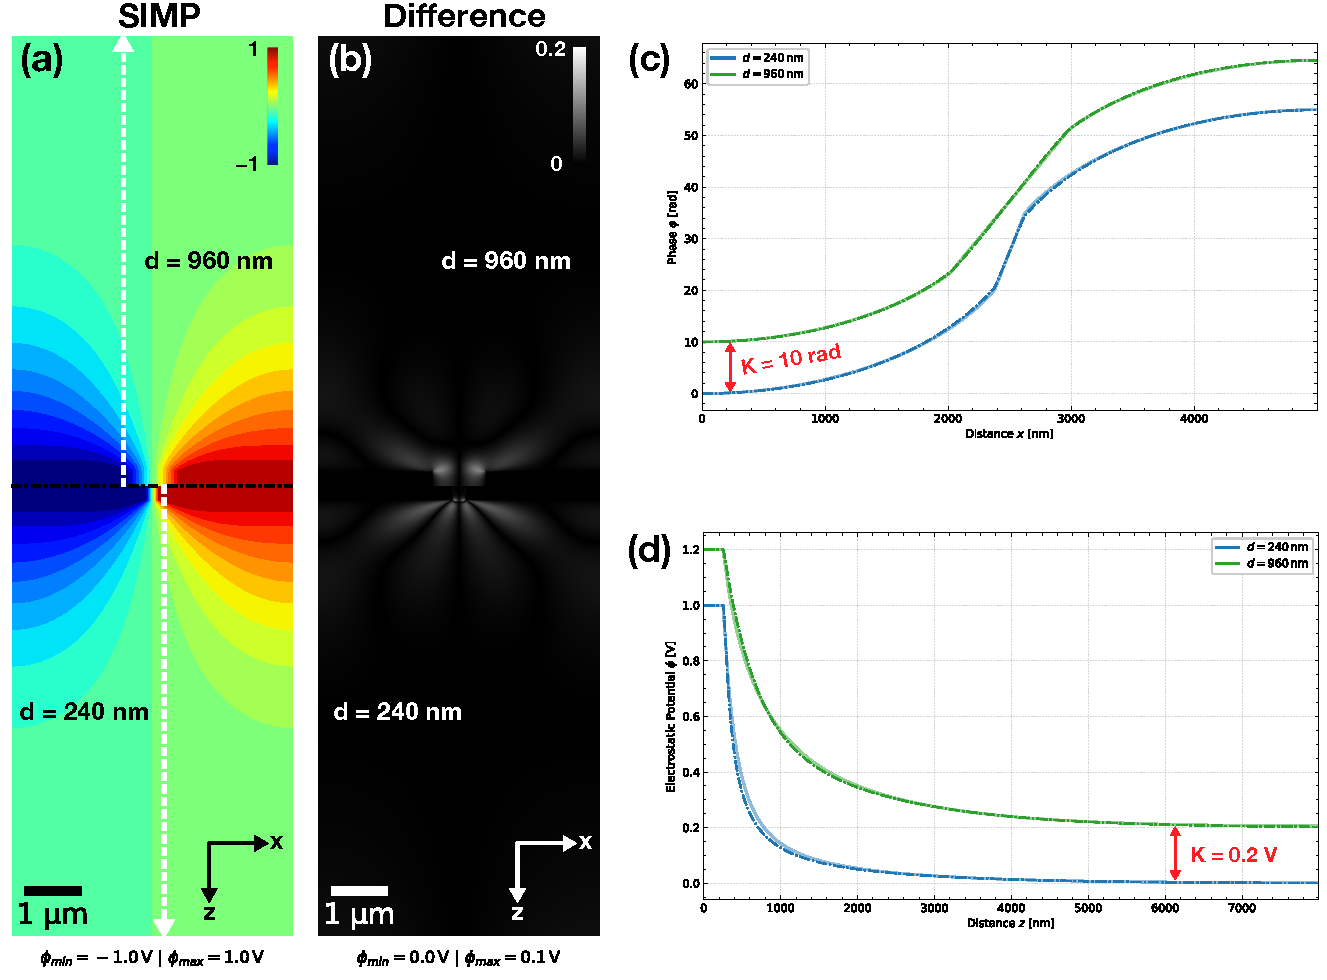
\includegraphics[width=\textwidth]{Figures/Results/Capacitor/Simulations/capacitor-FEM-SIMP-comparison-varying-distance.pdf}
	\caption{Comparison between the FEM simulation and \emph{SIMP} for the coplanar capacitor with (a) the 2D~electrostatic potential obtained from \emph{SIMP} for a distance between the capacitor plates of $d = \SI{960}{\nm}$ (upper half) and $d = \SI{240}{\nm}$ (lower half), their absolute differences in upper and lower half of (b), respectively, (c) the phases $\varphi$ obtained through a projection of the 2D~electrostatic potential $\phi$ and (d) the line profiles $\phi\left(z\right)$ of the electrostatic potential in propagation direction (indicated by the white dashed lines in a).}
	\label{fig:capacitor-FEM-SIMP-comparison-varying-distance}
\end{figure}
For the 2D~electrostatic potentials calculated from \emph{SIMP}, a behavior resembling the one mentioned above can also be observed for $d = \SI{960}{\nm}$ and $d = \SI{240}{\nm}$ (\cref{fig:capacitor-FEM-SIMP-comparison-varying-distance}a). Specifically, a modified specimen geometry with respect to the distance of the capacitor plates appears to result in negligible variations in the electrostatic potential beyond the immediate vicinity of the capacitor plate corners. For both plate distances, it can further be noted that the stray field extends far beyond the specimen edge into the vacuum. These minor variations in electrostatic potential due to modification of the specimen geometry are likewise reflected in the absolute difference between the FEM simulation and \emph{SIMP} (\cref{fig:capacitor-FEM-SIMP-comparison-varying-distance}b), where for both plate distances the maximum deviation does not exceed the previously observed value of $\Delta \phi_{\mathit{max}} = \SI{0.1}{\volt}$ and is likewise only located close to the contacts.

As with the original specimen geometry, the phase $\varphi$ can be calculated for both plate distances from a projection of the electrostatic potential (\cref{fig:capacitor-FEM-SIMP-comparison-varying-distance}c). For both plate distances $d = \SI{960}{\nm}$ and $d = \SI{240}{\nm}$ it is apparent that the FEM simulation and \emph{SIMP} are still in excellent agreement. The same observation is supported by the line profiles $\phi\left(z\right)$ of the electrostatic potential in propagation direction (\cref{fig:capacitor-FEM-SIMP-comparison-varying-distance}d, indicated by the white dashed lines in \cref{fig:capacitor-FEM-SIMP-comparison-varying-distance}a), where both line profiles likewise approach $\lim_{z\to\SI{8000}{\nm}} \phi\left(z\right) = \SI{0}{\volt}$.

In order to improve the visibility of the plotted phases, the phase for $d = \SI{240}{\nm}$ was offset to zero through subtraction by the first value, while the phase for $d = \SI{960}{\nm}$ was offset to $K = \SI{10}{rad}$. The same adjustments was made for the line profiles of the electrostatic potential, where the line profile for $d = \SI{960}{\nm}$ was offset by $K = \SI{0.2}{\volt}$ relative to line profile for $d = \SI{240}{\nm}$.

These preliminary findings (utilizing the coplanar capacitor as a reference specimen) suggest that \emph{SIMP} is a simple, yet promising, approach for the approximate modeling of electrostatic potential distributions. In order to verify the validity of the model, however, further comparisons with real-world measurements are needed, as detailed in the following \cref{ssec:experimental-results-SIMP-EH-comparison,ssec:capacitor-SIMP-tomography-comparison}.
\newpage
\subsection{Comparison with Off-Axis Electron Holography} \label{ssec:experimental-results-SIMP-EH-comparison}
Similar to \cref{ssec:experimental-results-capacitor-FEM-simulation}, comparisons are made with the experimentally obtained data described in \cref{ssec:experimental-results-capacitor-EH} (\cref{fig:capacitor-SIMP-EH-linescan-comparison}). Here, the object wave $\varphi_{\mathit{obj}}$ corresponds to the vacuum region between the contacts (\cref{fig:capacitor-FEM-SIMP-linescan-comparison}a, indicated by the dashed orange lines) and the reference wave $\varphi_{\mathit{ref}}$ to a region of the same size offset $\SI{800}{\nm}$ to the right (\cref{fig:capacitor-FEM-SIMP-linescan-comparison}a, indicated by the dashed red lines).
\begin{figure}[H]
	\centering
	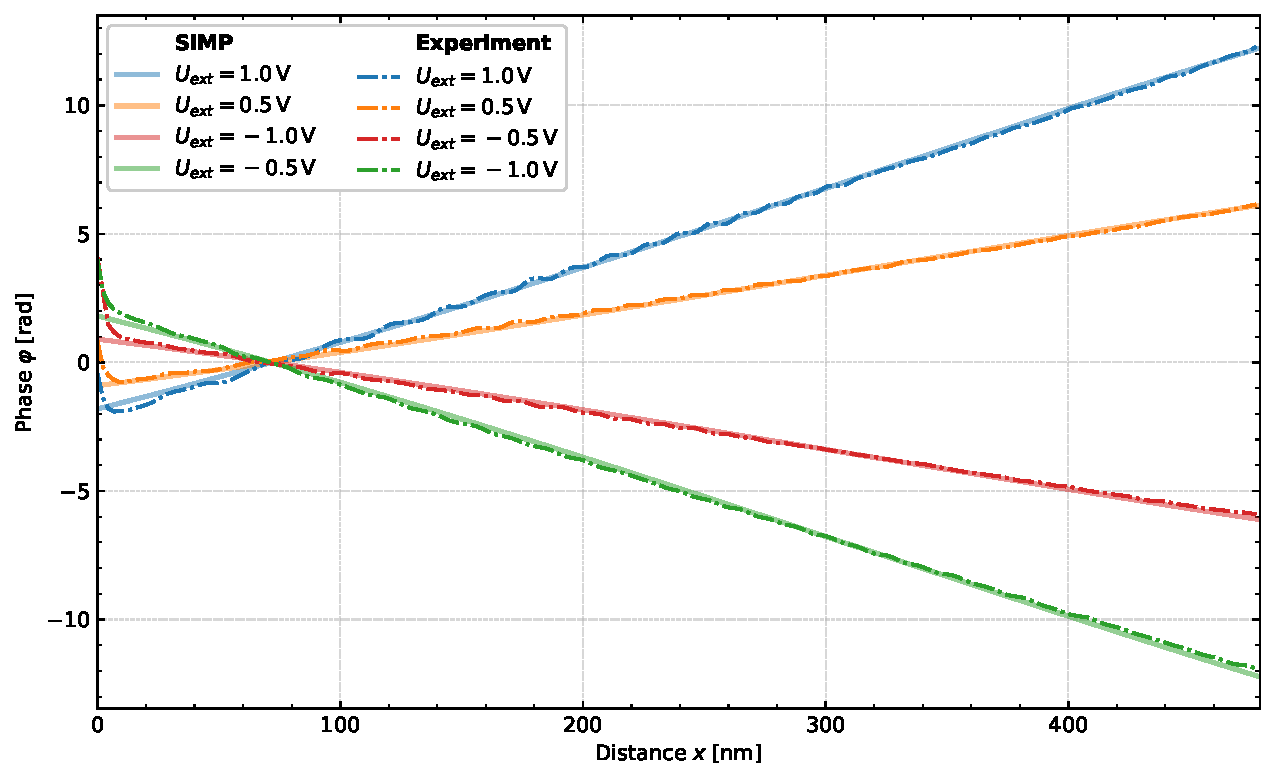
\includegraphics[width=\textwidth]{Figures/Results/Capacitor/Simulations/capacitor-SIMP-EH-linescan-comparison.pdf}
	\caption{Comparison between the phases $\varphi$ obtained from the experimentally acquired holograms (dashdotted lines) and those calculated with \emph{SIMP} (solid lines) for different bias voltages, where the reference wave $\varphi_{\mathit{ref}}$ is subtracted from the object wave $\varphi_{\mathit{obj}}$ according to the regions illustrated in \cref{fig:capacitor-FEM-SIMP-linescan-comparison}.}
	\label{fig:capacitor-SIMP-EH-linescan-comparison}
\end{figure}
As is the case with the FEM simulation, the simulated phases $\varphi$ obtained from \emph{SIMP} are in excellent agreement with the experimental phases acquired through off-axis EH for all external bias voltages $U_{\mathit{ext}}$, ranging from $\SIrange{-1.0}{1.0}{\volt}$ in increments of $\SI{0.5}{\volt}$, further supporting the validity of the proposed model.\footnote{Since the simulated coplanar capacitor was electrically biased by applying $\pm U_{\mathit{ext}}$ at the contacts, while the experimentally measured capacitor was grounded at one of the contacts, a scaling factor of $2$ has been applied when calculating the phase through projection.}

As before, the experimentally acquired 2D~phase images were modulated by subtracting a phase wedge (\cref{eq:holosuite-phase-wedge,eq:holosuite-phase-wedge-average-fit}).
\newpage
\subsection{Comparison with Electron Tomography} \label{ssec:capacitor-SIMP-tomography-comparison}
Due to its ability to obtain detailed structures of the investigated specimen in propagation direction, (electron) tomographic reconstruction represents a powerful measurement technique (a detailed description of the mathematical foundation behind (electron) tomography is given in \cref{sec:electron-tomography}). To be precise, the ability to obtain $n$-dimensional phase maps from $k$ $\left(n - 1\right)$ dimensional phase images (\cref{fig:TEM-tomography-capacitor-setup}) opens the door for the investigation of 3D~electric and magnetic properties of specimens on the nanometer scale and below.
\begin{figure}[H]
	\centering
	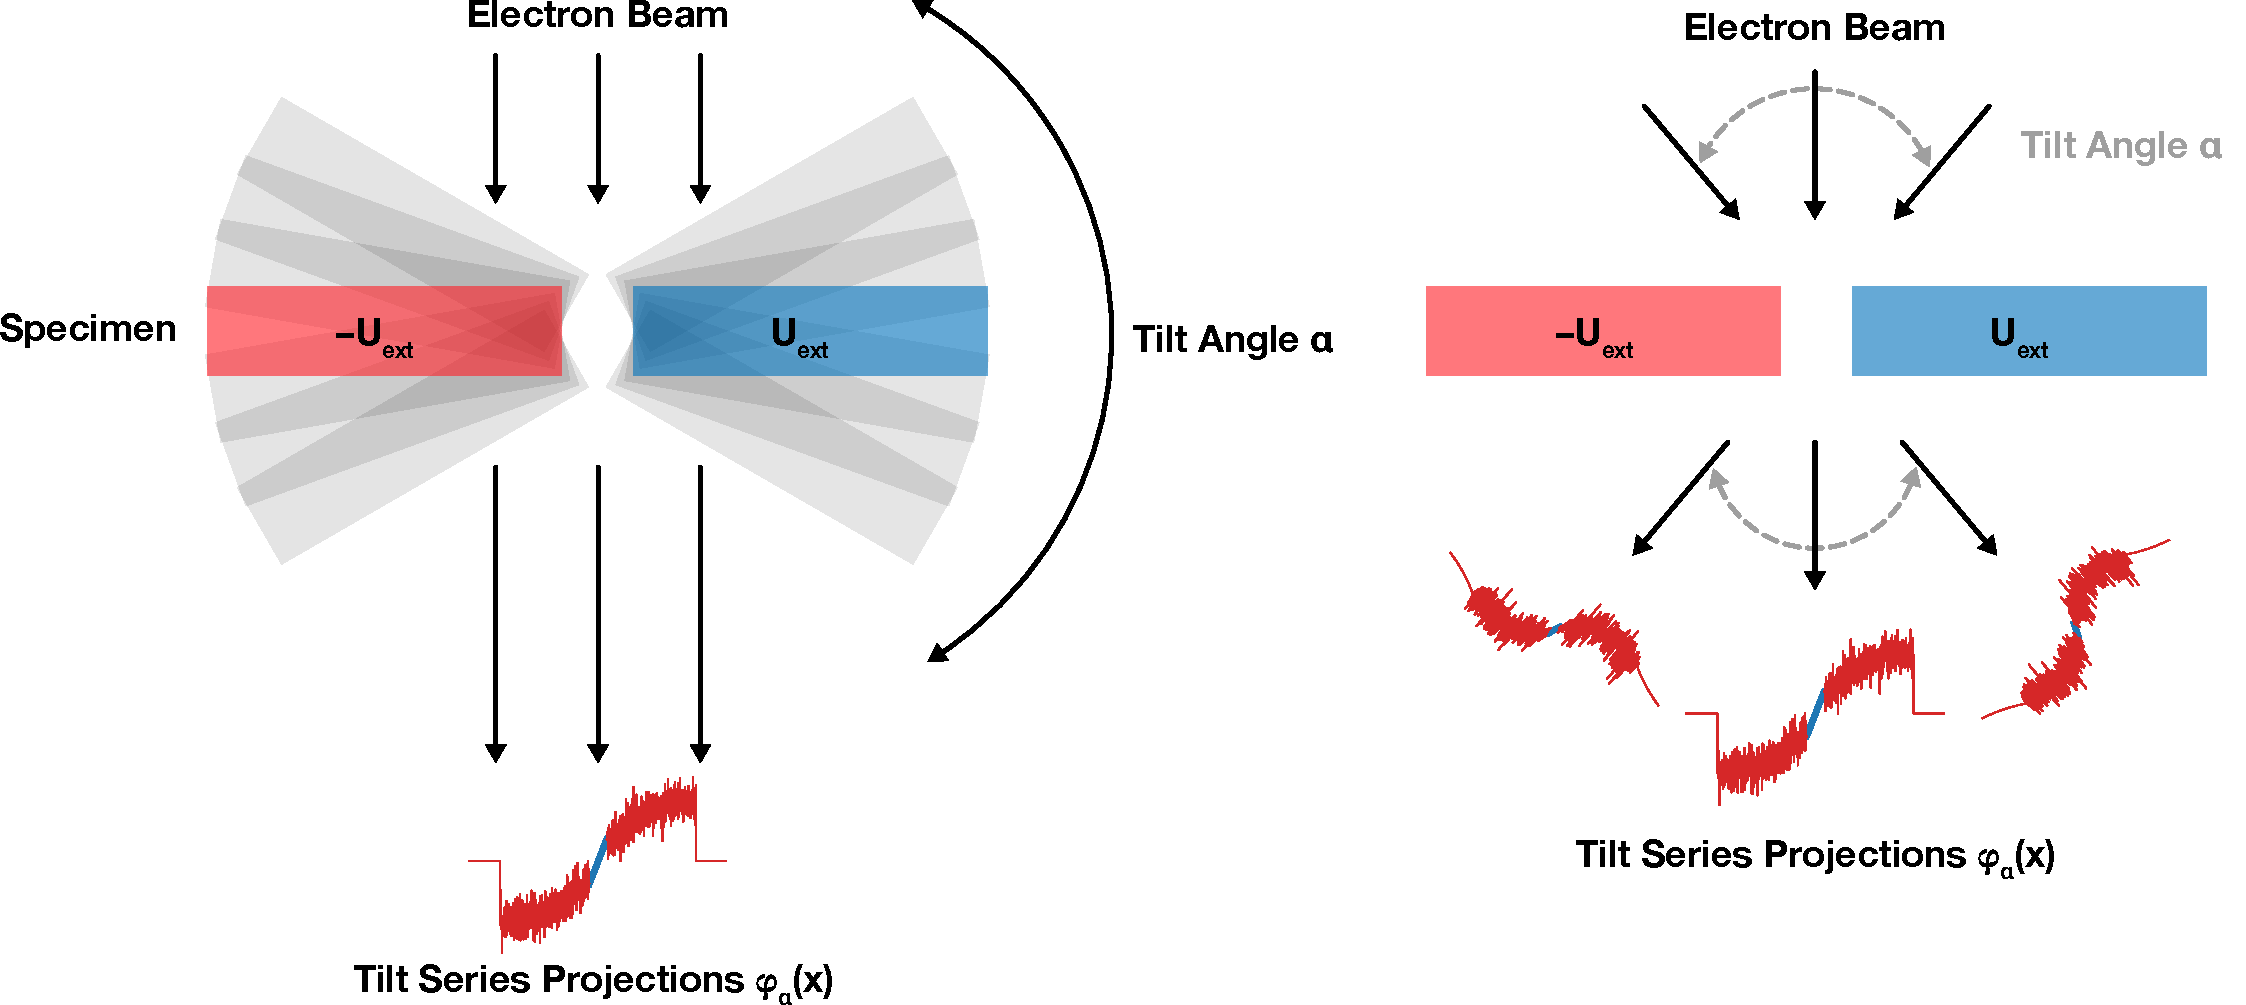
\includegraphics[width=\textwidth]{Figures/Schematics/Theoretical Foundations/TEM-tomography-capacitor-setup.pdf}
	\caption{Schematic illustration of the tomographic measurement process of the coplanar capacitor. The electron beam propagates through the specimen, which is rotated by a tilt angle $\alpha$, and generates the tilt series projection $\varphi_{\alpha}\left(x\right)$ on the detector. Since the capacitor plates are non-transparent, they cast a shadow on the detector when projected, necessitating that these areas of the projection be zeroed (illustrated by the red lines in the tilt series projections) so that the information between the electrodes (illustrated by the blue lines in the tilt series projections) remains.}
	\label{fig:TEM-tomography-capacitor-setup}
\end{figure}
In electron holographic tomography, by tilting the coplanar capacitor, a 2D~electron hologram is recorded for each tilt angle $\alpha$ (\cref{fig:TEM-tomography-capacitor-setup}), which is subsequently reconstructed as described in \cref{ssec:holosuite-automated-reconstruction}. For the phase images $\varphi$ obtained from this, a line profile between the capacitor plates is calculated for each of them as described in \cref{ssec:experimental-results-capacitor-EH}, where the composition of these 1D~line profiles $\varphi_{\alpha}\left(x\right)$ yields the 2D~sinogram $\hat{f}\left(\alpha, \varphi\right)$. In the case of the simulated 2D~electrostatic potential distributions, the 1D~line profiles follow directly from the projection through the Radon transform. The line profiles are subsequently offset to zero by subtracting their center value. Furthermore, all line profiles are zeroed in the area corresponding to the capacitor plates, reflecting the shadow the contacts cast due to their thickness (\cref{fig:TEM-tomography-capacitor-setup}, illustrated by the red lines in the tilt series projections). To do so, a linear fit between the capacitor plates is calculated and extrapolated to the whole projection, from which the capacitor plate edges can be detected with a threshold value for the deviation from the line profiles.
\newpage
In order to compare the above detailed results obtained from \emph{SIMP} with tomographically reconstructed phase images, the validity of the underlying Radon transform (\cref{eq:2D-radon-transform}) applied to the coplanar capacitor has to be verified first. For this purpose, the 2D~electrostatic potential obtained from \emph{SIMP} is Radon transformed by means of projection in an angular range of $\alpha = \pm \SI{90}{\degree}$ in $\SI{1}{\degree}$ increments, where the resulting sinogram is inverse radon transformed (\cref{fig:capacitor-SIMP-tomography-comparison}).
\begin{figure}[H]
	\centering
	\includegraphics[width=\textwidth]{Figures/Results/Capacitor/Tomography/capacitor-SIMP-tomography-comparison.pdf}
	\caption{Tomographic reconstruction utilizing \emph{scikit-image}'s implementation \cite{Vanderwalt2014} of the Radon transform (\cref{eq:2D-radon-transform}) with (a) the 2D~electrostatic potential $\phi$ obtained from \emph{SIMP}, (b) the sinogram $\hat{f}\left(\alpha, \varphi\right)$ calculated through projection (with the input assumed to be zero outside the inscribed circle), (c) the resulting tomographically reconstructed 2D~electrostatic potential $\phi_{\mathit{rec}}$ and (d) the same tomographic reconstruction $\phi_{\mathit{rec}}^{\mathit{rest}}$ with real-world like limitations and a 2D~Gaussian blur of $\sigma_G = 4.0$ applied.}
	\label{fig:capacitor-SIMP-tomography-comparison}
\end{figure}
It is observed that the sinogram $\hat{f}\left(\alpha, \varphi\right)$ (\cref{fig:capacitor-SIMP-tomography-comparison}b) following from the 2D~electrostatic potential (\cref{fig:capacitor-SIMP-tomography-comparison}a) results in a 2D~electrostatic potential which is in excellent agreement with the initially provided potential distribution (\cref{fig:capacitor-SIMP-tomography-comparison}c). The low noise observed in some areas of the tomographic reconstruction is the result of reconstruction artifacts in the Fourier transform of the filtered back projection (FBP), where a ramp filter was used in this case.

These observations validate tomographic reconstruction as a suitable measurement and analysis technique for the specimens described here. Furthermore, they demonstrate that the FBP is sufficiently accurate to yield results that match the input potential distribution of these specimens (\cref{fig:capacitor-SIMP-tomography-linescan-comparison}), thereby alleviating the need for computationally expensive iterative reconstruction schemes.

However, since real-world measurements possess several limitations, it is of interest to see how these constraints affect the tomographic reconstruction of the same 2D~electrostatic potential. In detail, it is of interest how a restriction of the tilt series to an angular range of $\alpha = \pm \SI{34}{\degree}$ in $\SI{2}{\degree}$ increments as well as a zeroing of the projection in the region of the capacitor plates affects the tomographic reconstruction. To better approximate the behavior observed in the experimental measurements, the 2D~electrostatic potential inside the contacts of the coplanar capacitor is replaced with random noise, where the values are an order of magnitude larger than externally applied bias.
\begin{figure}[H]
	\centering
	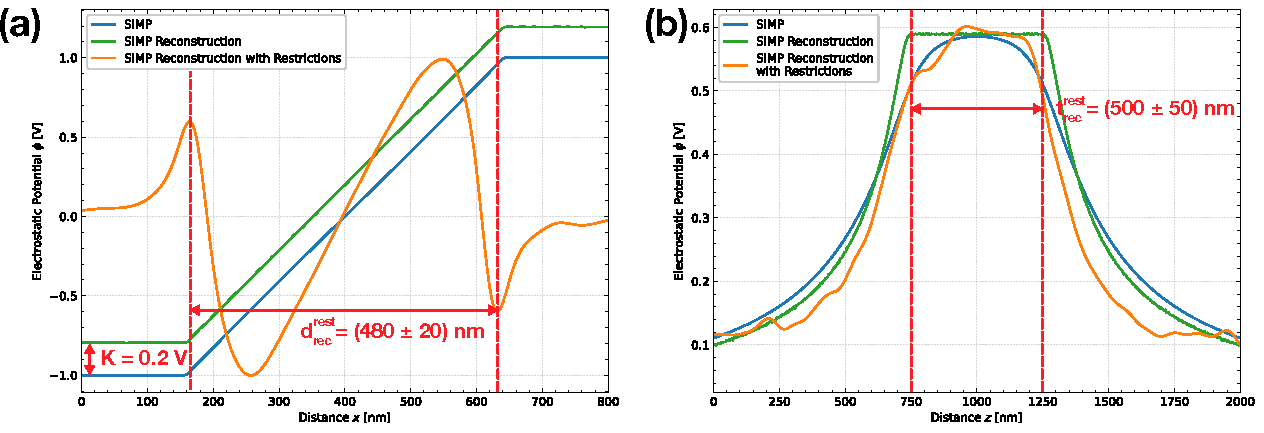
\includegraphics[width=\textwidth]{Figures/Results/Capacitor/Tomography/capacitor-SIMP-tomography-linescan-comparison.pdf}
	\caption{Comparison between the input 2D~electrostatic potential $\phi$ of the coplanar capacitor obtained from \emph{SIMP} and the tomographically reconstructed potential distributions $\phi_{\mathit{rec}}$ and $\phi_{\mathit{rec}}^{\mathit{rest}}$ with (a) the line profiles $\phi\left(x\right)$ across center of the specimen and (b) the line profiles $\phi\left(z\right)$ across the right contact (with both line profiles indicated by the solid and dashed white lines in \cref{fig:capacitor-SIMP-tomography-comparison}, respectively).}
	\label{fig:capacitor-SIMP-tomography-linescan-comparison}
\end{figure}
Here, it is apparent that the limited angular range of the tilt series (i.\,e.\ missing wedge) and the zeroing of the projection in the region of the capacitor plates (i.\,e.\ interior Radon transform) have a considerable impact on the tomographic reconstruction, which is especially noticeable in the limited spatial resolution in $z$-direction and almost completely missing information outside the region between the contacts (\cref{fig:capacitor-SIMP-tomography-comparison}d). Despite these severe limitations, the spacing of the capacitor plates can still be determined to be $d_{\mathit{rec}}^{\mathit{rest}} = \SI{480 \pm 20}{\nm}$ (\cref{fig:capacitor-SIMP-tomography-linescan-comparison}a, indicated by the red line) and the thickness of the specimen to be $t_{\mathit{rec}}^{\mathit{rest}} = \SI{500 \pm 50}{\nm}$ (\cref{fig:capacitor-SIMP-tomography-linescan-comparison}b, indicated by the red line), within whose measurement uncertainties the actual simulated values of $d = \SI{480}{\nm}$ and $t = \SI{500}{\nm}$ lie.

The deviation in slope as well as the ringing artifacts observed in the line profile of the restricted tomographic reconstruction $\phi_{\mathit{rec}}^{\mathit{rest}}\left(x\right)$ (\cref{fig:capacitor-SIMP-tomography-linescan-comparison}a) are likewise due to reconstruction artifacts arising from the previously mentioned real-world limitations (i.\,e.\ missing wedge, interior Radon transform and zeroing of the projection due to the shadow cast by the contacts).
\newpage
In order to improve the visibility of the plotted line profiles, the electrostatic potential $\phi_{\mathit{rec}}\left(x\right)$ obtained from the tomographic reconstruction of \emph{SIMP} without restrictions is offset by $K = \SI{0.2}{\volt}$.

These findings further suggest that the chosen angular resolution of $\Delta \alpha = \SI{2}{\degree}$ is sufficient enough to resolve the desired specimen features \cite{Yalisove2021}, where the achievable spacial resolution is given by the Crowther criterion \cite{Bracewell1967,Crowther1970}.

Having demonstrated the general validity of the tomographic reconstruction technique using the coplanar capacitor modeled with \emph{SIMP}, these results are compared to the tomographic reconstruction of the experimentally recorded holograms (\cref{fig:capacitor-SIMP-EH-tomography-comparison}).
\begin{figure}[H]
	\centering
	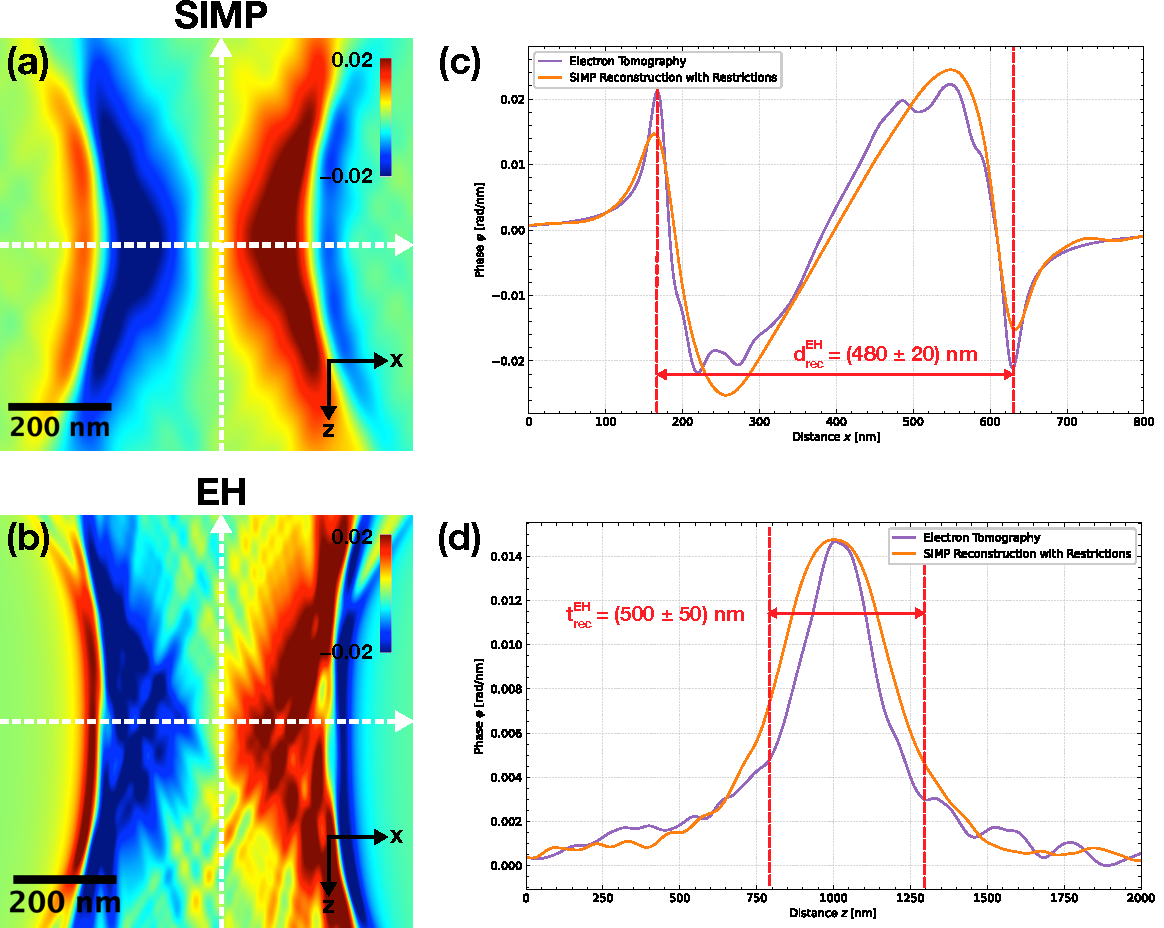
\includegraphics[width=\textwidth]{Figures/Results/Capacitor/Tomography/capacitor-SIMP-EH-tomography-comparison.pdf}
	\caption{Tomographic reconstruction of the coplanar capacitor with (a) the 2D~back-projected phase $\varphi_{\mathit{rec}}^{\mathit{rest}}$ obtained from \emph{SIMP}, (b) the 2D~back-projected phase $\varphi_{\mathit{rec}}^{\mathit{EH}}$ obtained from the experimentally acquired holograms, (c) the line profiles $\varphi\left(x\right)$ across the center of the specimen and (d) the line profiles $\varphi\left(z\right)$ across the right contact. For both 2D~back-projected phases, a 2D~Gaussian Blur of $\sigma_G = 4.0$ is applied.}
	\label{fig:capacitor-SIMP-EH-tomography-comparison}
\end{figure}
Considering the line profiles $\varphi\left(x\right)$, it is observed that, although the experimentally recorded data exhibits a noticeable degree of noise, the spacing of the capacitor plates can still be determined to be $d_{\mathit{rec}}^{\mathit{EH}} = \SI{480 \pm 20}{\nm}$ (\cref{fig:capacitor-SIMP-EH-tomography-comparison}c, indicated by the red line), which, accounting for the measurement uncertainty, is in agreement with the value obtained from \emph{SIMP}. The same applies to the line profiles $\varphi\left(z\right)$, where, despite the visible noise of the experimental data, the specimen thickness is determined to be $t_{\mathit{rec}}^{\mathit{EH}} = \SI{500 \pm 50}{\nm}$ (\cref{fig:capacitor-SIMP-EH-tomography-comparison}d, indicated by the red line), which, in the context of the measurement uncertainty, is in agreement with the value obtained from \emph{SIMP}. In general, both the 2D~back-projected phases (\cref{fig:capacitor-SIMP-EH-tomography-comparison}a and b) and the line profiles (\cref{fig:capacitor-SIMP-EH-tomography-comparison}c and d, indicated by the dashed white lines in \cref{fig:capacitor-SIMP-EH-tomography-comparison}a and b) showcase excellent agreement between the experimentally acquired holograms and the simulated specimen, further validating \emph{SIMP} as a suitable modeling approach for the approximation of electrostatic potential distributions.
\newpage
\section{Extension to Semiconductor Nanostructures}
After validating the underlying approach of the presented model in the previous \cref{sec:coplanar-capacitor-SIMP-EH-comparison} using the coplanar capacitor as a reference specimen, this chapter extends the presented model to semiconductor nanostructures using a multi-layer framework. This extension enables the study of the electrostatic potential distribution within doped semiconductor nanostructures and its impact on off-axis EH, providing valuable information for the characterization and optimization of such nanoscale electronic devices.
\subsection[\texorpdfstring{$p$-$n$}{\textit{p}-\textit{n}}-Junction]{$\boldsymbol{p}$-$\boldsymbol{n}$-Junction} \label{ssec:SIMP-pn-junction-extension}
One of the simplest semiconductor nanostructures is the symmetrically doped $p$-$n$-junction, which is used for didactical reasons. However, it should be noted that for comparison with experimental data, the previously introduced $p$-$p^+$-$n^+$-junction is used. For this, similar to the geometric layout described in \cref{ssec:2d-modeling-specimen}, two Si~specimen regions are defined and modeled, where both the $p$-region and the $n$-region are doped with $\SI[per-mode=power]{1e19}{\per\cubic\cm}$ and have a width of $\SI{2500}{\nm}$ and thickness of $\SI{150}{\nm}$ each. Outside the specimen, a vacuum region of $\SI{2500}{\nm}$ is assumed, with the overall geometry of the model being $\SI{5000}{\nm} \times \SI{2650}{\nm}$. The axial symmetry of the problem can again be exploited to reduce the computational complexity of the problem by modeling only half of the specimen's geometry.

Contrary to the coplanar capacitor, the initial electrostatic potential distribution $\phi_0\left(x\right)$ is not given by a constant potential at both contacts and a linear gradient in between, but rather by \cref{eq:pn-junction-potential}. With this initial electrostatic potential distribution, the 2D~electrostatic potential $\phi$, similar to the coplanar capacitor, can be calculated using \cref{eq:SIMP-electrostatic-potential-convolution}, where the standard deviation $\sigma_G$ of the projection distant dependent (normalized) 1D~Gaussian convolution kernel scales with a power of $\ln\left(2\right)$ outside the specimen (\cref{fig:pn-junction-SIMP-multilayer-EH-comparison}).

Comparing the 2D~electrostatic potential $\phi_{\mathit{SL}}$ obtained from \emph{SIMP} within the single-layer framework (\cref{fig:pn-junction-SIMP-multilayer-EH-comparison}a) with the experimentally acquired holograms of the $p^+$-$n^+$-junction through their phases $\varphi$ (i.\,e.\ a projection in propagation direction), it is apparent that the single-layer model fails to accurately describe the experimentally acquired holograms (\cref{fig:pn-junction-SIMP-multilayer-EH-comparison}d). Not only is the observable phase jump of the single-layer model more than twice as large as the experimentally acquired one, but the width of the depletion region $\omega$ (which follows from \cref{eq:depletion-region-width-n-region,eq:depletion-region-width-p-region}) obtained from \emph{SIMP} is also an order of magnitude smaller than the experimentally observed one.
\newpage
The primitive single-layer model, as is the case with the \emph{nextnano} simulations, assumes a specimen that has suffered no sub-surface preparation damage and is therefore not able to accurately describe the kinds of specimens investigated in a TEM. These observations consequently necessitate the need for a multi-layer framework that takes these various preparation damage effects into account while still requiring minimal knowledge about the microscopic charge carrier distribution.
\begin{figure}[H]
	\centering
	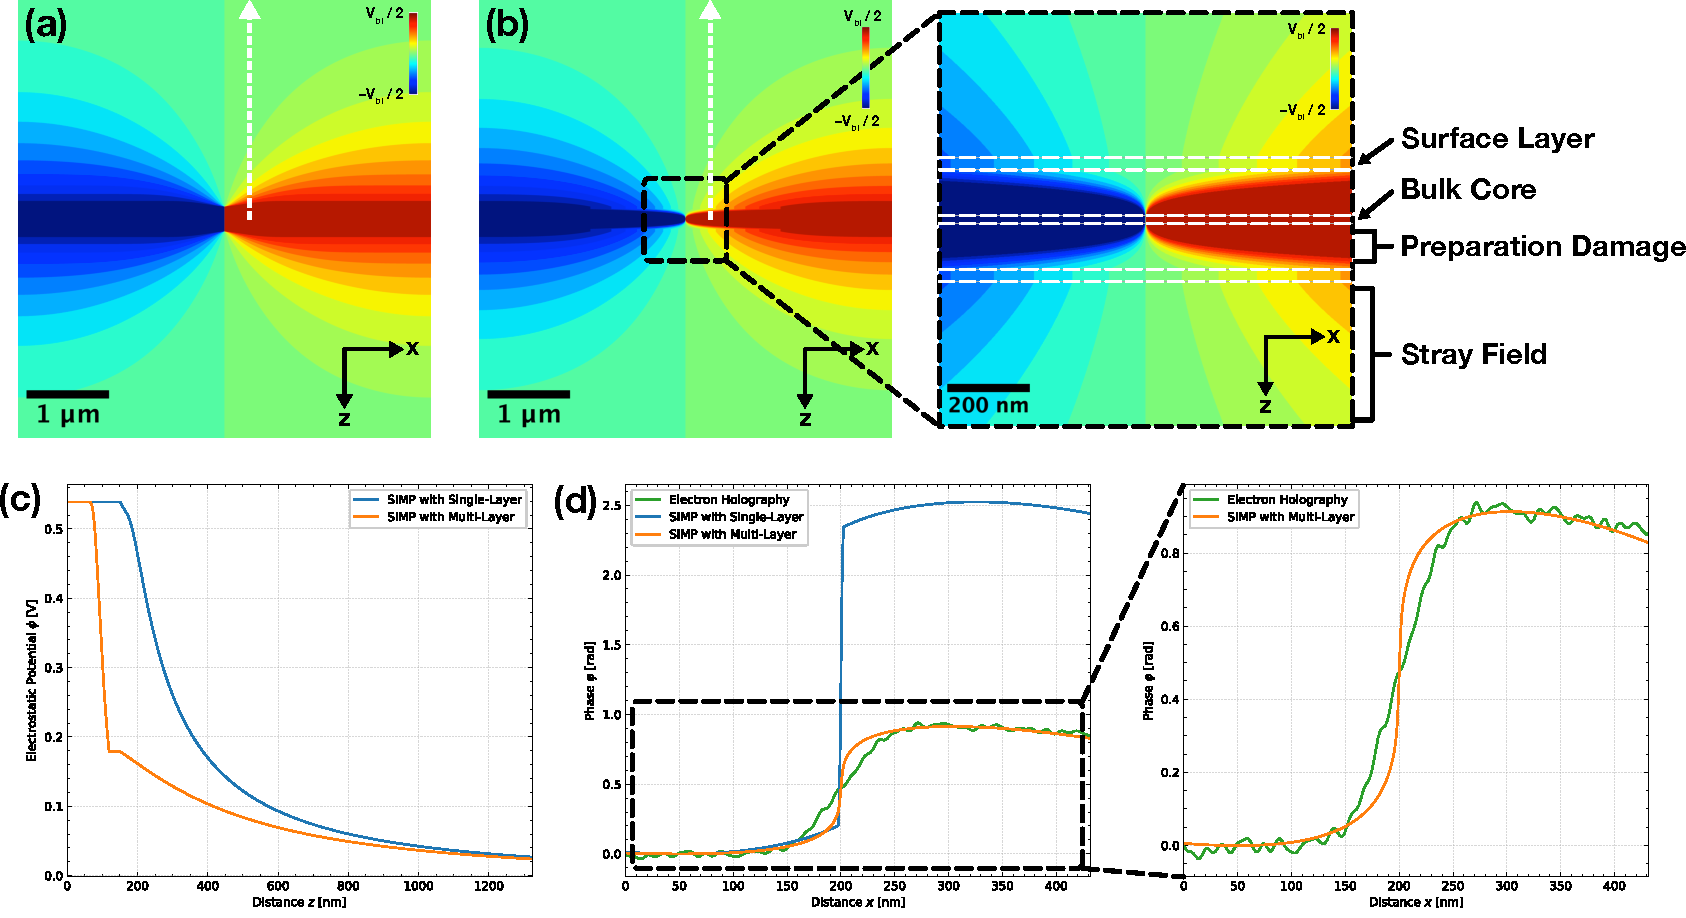
\includegraphics[width=\textwidth]{Figures/Results/pn-Junction/Simulations/pn-junction-SIMP-multilayer-EH-comparison.pdf}
	\caption{Comparison between the differently layered \emph{SIMP} frameworks for the symmetrically doped $p$-$n$-junction with (a) the 2D~electrostatic potential $\phi_{\mathit{SL}}$ obtained from the single-layer model, (b) the 2D~electrostatic potential $\phi_{\mathit{ML}}$ obtained from the multi-layer model, (c) the corresponding line profiles $\phi\left(z\right)$ in propagation direction (indicated by the white dashed lines in a and b) and (d) the phases $\varphi$ obtained through a projection of $\phi$ compared with the experimentally acquired holograms.}
	\label{fig:pn-junction-SIMP-multilayer-EH-comparison}
\end{figure}
As indicated in \cref{ssec:experimental-results-pnjunction-FEM-simulation}, the FIB preparation stage generates Ga-induced defects resulting in an electrically damaged crystalline layer below the electrically inactive surface layer \cite{Twitchett2002,Beleggia2003,Cooper2006,Cooper2007,Twitchett-Harrison2007,Cooper2009,Somodi2013,Yazdi2015}. As such, the specimen can be divided into three different regions:
\begin{itemize}
	\item \textbf{Bulk Core:} The 2D~electrostatic potential $\phi_{\mathit{ML}}$ follows the classical bulk theory for a $p$-$n$-junction (given by \cref{eq:pn-junction-potential}) and is given by the initial electrostatic potential distribution $\pdv*{\phi_0\left(x\right)}{z} = \text{const.}$;
	\item \textbf{Preparation Damage:} Here, the specimen suffers preparation damage due to the ion implantation by the FIB over an implantation depth $t_{\mathit{PD}}$. The degree of damage depends, among other things, on parameters such as the accelerating voltage $U_{\mathit{acc}}$ of the FIB and the atomic number $Z$ of the ions used for milling. The 2D~electrostatic potential $\phi_{\mathit{ML}}$ follows, similar to \cref{eq:SIMP-electrostatic-potential-convolution}, through a convolution of the bulk core potential distribution $\phi_0\left(x\right)$ with a projection distant dependent 1D~Gaussian kernel $G_{\mathit{1D}}\left(z\right)$;
	\item \textbf{Surface Layer:} This region represents an electrically inactive amorphous transition layer between the preparation damage region and the stray field. Here, the 2D~electrostatic potential $\phi_{\mathit{ML}}$ is given by the outer edge of the preparation damage layer $\pdv*{\phi_{t_{\mathit{PD}}}\left(x\right)}{z} = \text{const.}$
\end{itemize}
Given this multi-layer framework for \emph{SIMP}, a total of three distances have to be defined: The bulk core thickness $t_{\mathit{BC}}$, the implantation depth of the preparation damage region~$t_{\mathit{PD}}$ and the amorphous surface layer thickness $t_{\mathit{SL}}$.

The thickness of the amorphous surface layer $t_{\mathit{SL}}$ can be experimentally determined by comparing convergent-beam electron diffraction (CBED) measurements with off-axis EH measurements (\cref{fig:CBED-comparison-simulation-thickness}, a detailed description of CBED can be found in \cref{chap:appendix-CBED}). In detail, the crystalline part of the specimen thickness is determined to be $t_{\mathit{CBED}} = \SI{270 \pm 2}{\nm}$, where the difference to the thickness of $t_{\mathit{EH}} = \SI{325 \pm 5}{\nm}$ measured with off-axis EH (\cref{chap:appendix-specimen-thickness-off-axis-EH}) yields the surface layer thickness of $t_{\mathit{SL}} = \SI{30 \pm 5}{\nm}$.

Using a surface layer thickness of $t_{\mathit{SL}} = \SI{30}{\nm}$ and a bulk core thickness of $t_{\mathit{BC}} = \SI{10}{\nm}$, the preparation damage region has a thickness of $t_{\mathit{PD}} = \SI{110}{\nm}$. With this, along with the same parameters for the stray field as before, the 2D~electrostatic potential~$\phi_{\mathit{ML}}$ can be calculated (\cref{fig:pn-junction-SIMP-multilayer-EH-comparison}b). The single-layer model and multi-layer model can then be compared through their corresponding line profiles $\phi\left(z\right)$ in propagation direction (indicated by the white dashed lines in \cref{fig:pn-junction-SIMP-multilayer-EH-comparison}a and b), where it is apparent that, while both models match inside the bulk core region (i.\,e.\ for $\lvert z \rvert \leq t_{\mathit{BC}}$) and approach $\lim_{z\to\SI{2650}{\nm}} \phi\left(z\right) = \SI{0}{\volt}$, the preparation damage region introduced in the multi-layer model causes the electrostatic potential distribution to decay considerable earlier compared to the single-layer model (\cref{fig:pn-junction-SIMP-multilayer-EH-comparison}c). Furthermore, by comparing the phase $\varphi$ of the multi-layer model (obtained through a projection of the electrostatic potential in propagation direction) to the experimentally acquired holograms, it is apparent that the multi-layer framework is in significantly greater agreement with the real-world measurements (\cref{fig:pn-junction-SIMP-multilayer-EH-comparison}d).

As described in \cref{ssec:FEM-simulated-potential-and-phase} the phases $\varphi$ obtained from \emph{SIMP} are calculated by subtracting the reference phase $\varphi_{\mathit{ref}}$, which only contains the stray field contribution, from the object phase $\varphi_{\mathit{obj}}$ (where both are separated by the biprism shadow) and modulating them through the subtraction of a phase wedge.
\newpage
\subsection[\texorpdfstring{$p$-$p^+$-$n^+$}{\textit{p}-\textit{p}\textsuperscript{+}-\textit{n}\textsuperscript{+}}-Junction]{$\boldsymbol{p}$-$\boldsymbol{p^+}$-$\boldsymbol{n^+}$-Junction} \label{ssec:SIMP-ppn-junction-extension}
Having established the validity of the multi-layer framework for \emph{SIMP} using a symmetrically doped $p$-$n$-junction in the previous \cref{ssec:SIMP-pn-junction-extension}, the same multi-layer model can now be extended to a $p$-$p^+$-$n^+$-junction.

For this, a Si~specimen with an geometric layout identical to \cref{fig:specimen-nextnano-layout} is modeled, where each doped region has a width of $\SI{1000}{\nm}$ and a thickness of $\SI{150}{\nm}$. The vacuum region outside the specimen extends for $\SI{2500}{\nm}$, for a total geometry of $\SI{3000}{\nm} \times \SI{2650}{\nm}$. As with the previous simulations, the axial symmetry of the problem is exploited to reduce the computational complexity of the simulation.

Identical to the above described specimen, the initial electrostatic potential distribution~$\phi_0 \left(x\right)$ at the junction between the $p^+$-region and $n^+$-region, which are both doped with $\SI[per-mode=power]{1e19}{\per\cubic\cm}$, is given by \cref{eq:pn-junction-potential}. The weakly doped (i.\,e.\ $\SI[per-mode=power]{1e16}{\per\cubic\cm}$) $p$-region causes the formation of another depletion region similar to the $p^+$-$n^+$-junction, where the fundamental mechanism is likewise described by \cref{eq:pn-junction-potential} but with different boundary conditions \cite{Sabnis1978}.

With this modified initial potential distribution~$\phi_0 \left(x\right)$, where all other parameters with respect to the different thicknesses of the specimen regions and the 1D~Gaussian convolution kernel are kept the same, the 2D~electrostatic potential~$\phi_{\mathit{ML}}$ can be obtained from \emph{SIMP} (\cref{fig:ppn-junction-SIMP-multilayer-EH-comparison}).
\begin{figure}[H]
	\centering
	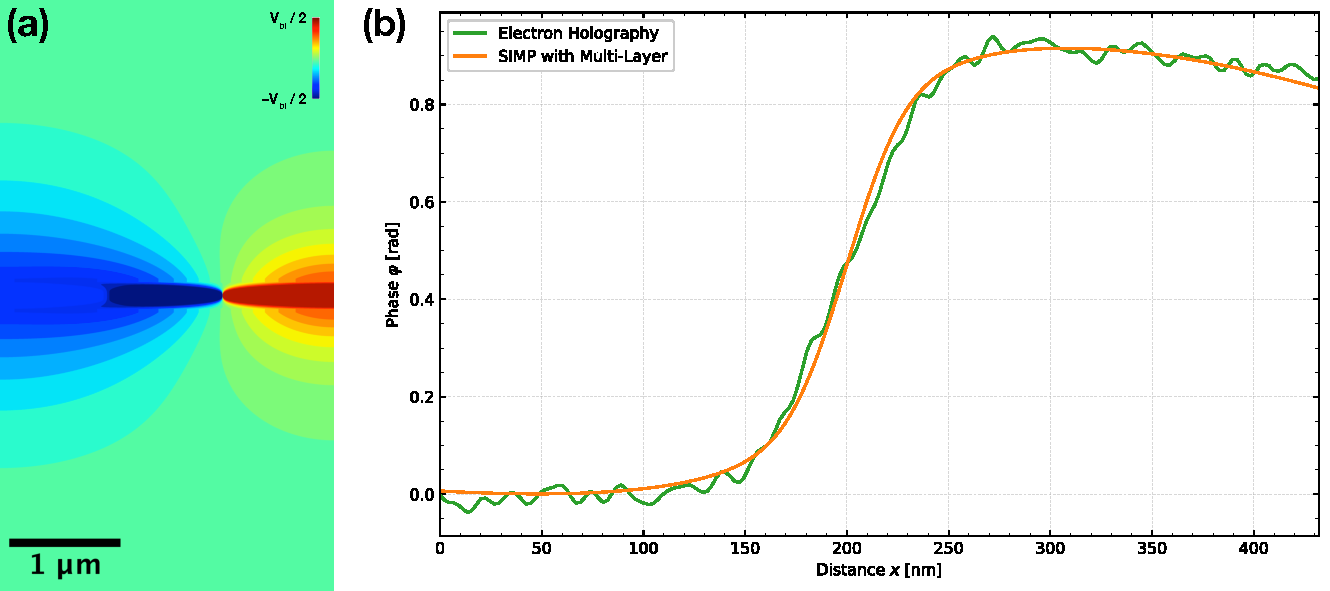
\includegraphics[width=\textwidth]{Figures/Results/pn-Junction/Simulations/ppn-junction-SIMP-multilayer-EH-comparison.pdf}
	\caption{Comparison between the multi-layer framework for \emph{SIMP} and off-axis EH with for the $p$-$p^+$-$n^+$-junction with (a) the 2D~electrostatic potential~$\phi_{\mathit{ML}}$ calculated through the above described multi-layer model and parameters and (b) the phases $\varphi$ obtained through a projection of $\phi$ in propagation direction.}
	\label{fig:ppn-junction-SIMP-multilayer-EH-comparison}
\end{figure}
By comparing the phases $\varphi$ obtained through a projection of the 2D~electrostatic potential~$\phi$ in propagation direction, it is apparent that the same multi-layer framework for \emph{SIMP} is still in great agreement with the experimentally acquired holograms (\cref{fig:ppn-junction-SIMP-multilayer-EH-comparison}b). This is particularly evident when compared to the phases obtained from the \emph{nextnano} simulations, which exhibit large deviations compared to the experimentally acquired holograms (\cref{fig:pn-junction-FEM-EH-linescan-comparison}c). Furthermore, by applying a spatial filter (i.\,e.\ 1D~Gaussian filter) which is equivalent to the mask radius chosen when reconstructing the experimentally acquired electron waves, the phase $\varphi\left(x\right)$ obtained from \emph{SIMP} is in excellent agreement with the experimentally acquired holograms (\cref{fig:ppn-junction-SIMP-multilayer-EH-comparison}b). Additionally, the $p$-$p^+$-junction has no significant influence on the projected electrostatic potential of the $p^+$-$n^+$-junction.

Similar to \cref{ssec:capacitor-SIMP-tomography-comparison}, both the experimentally acquired holograms and the multi-layer \emph{SIMP} framework are tomographically reconstructed and compared for an externally applied bias of $U_{\mathit{ext}} = \SI{2.0}{\volt}$ (\cref{fig:ppn-junction-SIMP-EH-tomography-comparison}). Here, experimentally acquired holograms of the unbiased specimen (i.\,e.\ $U_{\mathit{ext}} = \SI{0}{\volt}$) are used for normalization during the numerical reconstruction process, therefore removing unwanted phase modulations (e.\,g.\ surface charging) and yielding only the change caused by the externally applied bias \cite{Wagner2019}.
\begin{figure}[H]
	\centering
	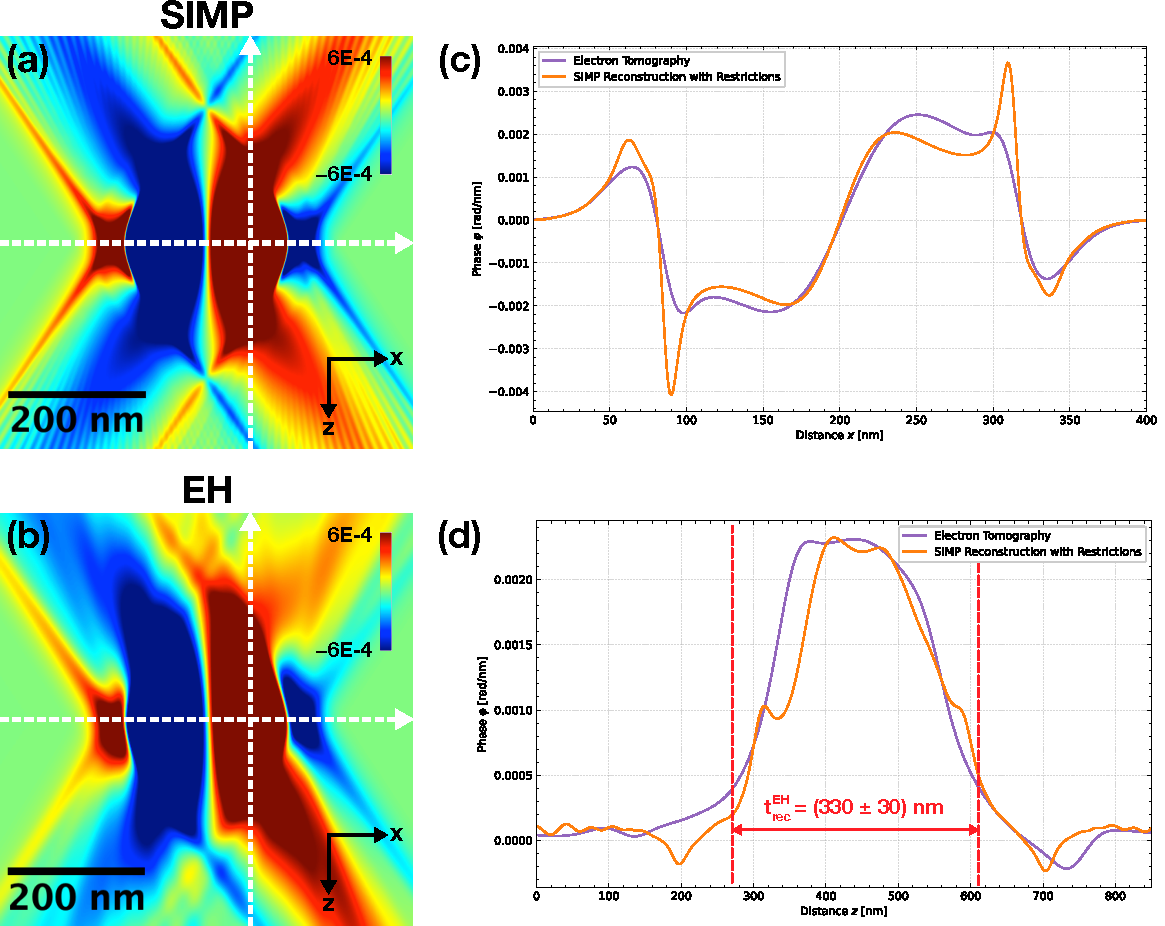
\includegraphics[width=\textwidth]{Figures/Results/pn-Junction/Tomography/ppn-junction-SIMP-EH-tomography-comparison.pdf}
	\caption{Tomographic reconstruction of the $p$-$p^+$-$n^+$-junction with (a) the 2D~back-projected phase $\varphi_{\mathit{rec}}^{\mathit{rest}}$ obtained from the multi-layer \emph{SIMP} framework, (b) the 2D~back-projected phase $\varphi_{\mathit{rec}}^{\mathit{EH}}$ obtained from the experimentally acquired holograms, (c) the line profiles $\varphi\left(x\right)$ across the center of the specimen and (d) the line profiles $\varphi\left(z\right)$ across the $n^+$-region for an externally applied bias of $U_{\mathit{ext}} = \SI{2.0}{\volt}$. For both 2D~back-projected phases, a 2D~Gaussian Blur of $\sigma_G = 4.0$ is applied.}
	\label{fig:ppn-junction-SIMP-EH-tomography-comparison}
\end{figure}
Considering the lines profiles $\varphi\left(z\right)$ (indicated by the white dashed lines in \cref{fig:ppn-junction-SIMP-EH-tomography-comparison}a and b), it is observed that both specimen thicknesses obtained from the multi-layer \emph{SIMP} framework and the experimentally acquired holograms are determined to be $t_{\mathit{rec}}^{\mathit{rest}} = t_{\mathit{rec}}^{\mathit{EH}} = \SI{330 \pm 30}{\nm}$, where both lines profiles are in excellent agreement (\cref{fig:ppn-junction-SIMP-EH-tomography-comparison}d). Despite the strongly restricted angular range of the tomographic tilt series, resulting in a limited spatial resolution in $z$-direction, a considerable reduction in the width of the potential jump located at a central region of specimen (far from the specimen surfaces) is observed in comparison with the classical reconstructed phase (\cref{fig:ppn-junction-SIMP-EH-tomography-comparison}c).

These results further corroborate the validity of the multi-layer framework for \emph{SIMP}, where the bulk core region only contributes a small part to the overall phase and the preparation damage layer caused by the FIB extends deep into the specimen. Furthermore, the multi-layer system determined through \emph{SIMP} is in excellent agreement with the specimen thickness previously obtained through the comparison between off-axis EH and CBED.

The deviations observed towards the edges of the specimen between the experimentally acquired holograms and the multi-layer framework for \emph{SIMP} for the line profiles $\varphi\left(x\right)$ (indicated by the white dashed lines in \cref{fig:ppn-junction-SIMP-EH-tomography-comparison}a and b) can again be attributed to reconstructing artifacts in the FBP. Additionally, the slight asymmetry between the $p^+$-region and $n^+$-region of the experimentally acquired holograms can potentially be attributed, among other things, to a non-zero pre-tilt of the specimen inside the holder, electron beam induced charging of the specimen surface (which is different for the $p^+$-region and $n^+$-region) or the built-up of a surface current when applying an external bias voltage to the specimen (i.\,e.\ shunt resistance).

Similar to the experimentally acquired holograms, the phases $\varphi$ are calculated through the projection of the 2D~electrostatic potential $\phi_{\mathit{ML}}$ obtained from \emph{SIMP} for every tilt angle $\alpha \in \left\{\SI{-34}{\degree}, \SI{-32}{\degree}, \dots , \SI{+32}{\degree}, \SI{+34}{\degree}\right\}$, where a cutout of similar size to the field of view is centered around the depletion region, and modulated through the subtraction of a linear fit, ranging from 10\% to 20\% and extrapolated to the entire field of view, from all values (\cref{ssec:FEM-simulated-potential-and-phase}).

To ensure comparability between \emph{SIMP} and the experimentally measured holograms, the phases for no externally applied bias (i.\,e.\ $U_{\mathit{ext}} = \SI{0}{\volt}$) must be subtracted for the multi-layer framework, as was the case for the experimentally measured $p$-$p^+$-$n^+$-junction. Due to the abnormal switching behavior of the specimen, which is in part caused by the built-up of an Schottky barrier, the increase in the phase jump $\Delta \varphi\left(x\right)$ is not given by \cref{eq:pn-junction-potential}, which would predict a phase jump of $\Delta \varphi\left(x\right) \approx \SI{3.1}{\volt}$, but rather by the considerably smaller change observed in \cref{ssec:experimental-results-ppn-junction-off-axis-EH} (\cref{fig:pn-junction-off-axis-EH-phase-jump}b). After subtracting the phases for no externally applied bias, a spatial filter (i.\,e.\ 1D~Gaussian filter) equivalent to the mask radius chosen when reconstructing the experimentally acquired electron waves is applied.

\emph{SIMP} therefore allows for the approximation of the electrostatic potential distribution in electrically biased complex real-world specimens, especially with regards to the propagation direction of the electron beam, through a limited set of parameters obtained by comparison with only one reconstructed phase.
